% !TeX spellcheck = en_US
% !TeX encoding = UTF-8
\documentclass{beamer}

\mode<presentation> { \usetheme{Madrid} }

\usepackage{graphicx, graphics}
\usepackage[notocbib]{apacite}
\usepackage[style=iso]{datetime2}
\usepackage{enumerate}
\usepackage[T1]{fontenc}
\usepackage{booktabs}
\providecommand\thispdfpagelabel[1]{}
\DeclareGraphicsExtensions{.pdf, .png, .jpg, .gif}

\AtBeginSection[]
{
    \begin{frame}
        \vfill
        \centering
        \begin{beamercolorbox}[sep=8pt,center,shadow=true,rounded=true]{title}
            \usebeamerfont{title}
            \thesection. \insertsectionhead
            \par
        \end{beamercolorbox}
        \vfill
    \end{frame}
}

\AtBeginSubsection[]
{
    \begin{frame}
        \vfill
        \centering
        \begin{beamercolorbox}[sep=8pt, center, shadow=true, rounded=true]{title}
            \usebeamerfont{title}
            \thesection. \insertsectionhead
            \par
        \end{beamercolorbox}
        \begin{beamercolorbox}[sep=6pt, center, shadow=true, rounded=true]{title}
            \usebeamerfont{subtitle}
            \thesection.\thesubsection. \insertsubsectionhead
            \par
        \end{beamercolorbox}
        \vfill
    \end{frame}
}

\AtBeginSubsubsection[]
{
    \begin{frame}
        \vfill
        \centering
        \begin{beamercolorbox}[sep=8pt, center, shadow=true, rounded=true]{title}
            \usebeamerfont{title}
            \thesection. \insertsectionhead
            \par
        \end{beamercolorbox}
        \begin{beamercolorbox}[sep=6pt, center, shadow=true, rounded=true]{title}
            \usebeamerfont{subtitle}
            \thesection.\thesubsection. \insertsubsectionhead
            \par
        \end{beamercolorbox}
        \begin{beamercolorbox}[sep=4pt, center, shadow=true, rounded=true]{title}
            \usebeamerfont{subsubtitle}
            \thesection.\thesubsection.\thesubsubsection. \insertsubsubsectionhead
            \par
        \end{beamercolorbox}
        \vfill
    \end{frame}
}

\title[PTB]{Metagenome Analysis of Preterm Birth}

\author[Jaewoong Lee]
{
    Jaewoong Lee
    \and
    Semin Lee
}

\institute[UNIST BME]
{
    Department of Biomedical Engineering
    \newline
    Ulsan National Institute of Science and Technology
    \medskip
    \newline
    \textit{jwlee230@unist.ac.kr}
}

\date{\today}

\begin{document}
    \begin{frame}
        \titlepage
    \end{frame}

	\begin{frame}
        \frametitle{Overview}
        \tableofcontents[hideallsubsections]
    \end{frame}

    \section{Introduction}
    \begin{frame}
        \frametitle{Microbiome}

        \begin{itemize}
            \item Microbiota: the microorganisms which live inside \& on humans \cite{micro1}
            \item Microbiome: $10^{13}$ to $10^{14}$ microorganisms whose which collective genome \cite{micro2}
        \end{itemize}

        \begin{figure}
            \includegraphics[width=0.3 \linewidth]{figures/microbiome.jpg}
            \caption{Concept of a core human microbiome \protect \cite{micro1}}
        \end{figure}
    \end{frame}

    \begin{frame}
        \frametitle{rRNA}

        \begin{itemize}
            \item Ribosomal RNA
            \item Well-known as a key to phylogeny \cite{rrna1}
        \end{itemize}
    \end{frame}

    \begin{frame}
        \frametitle{Preterm Birth (PTB)}

        PTB:
        \begin{enumerate}
            \item PTB $<$ 37 GW (Gestational week)
            \item Normal $\ge$ 37 GW
        \end{enumerate}

        \cite{premature1, premature2}
    \end{frame}

    \section{Materials}
    \begin{frame}
        \frametitle{16S rRNA Sequencing}

        \textbf{16S rRNA sequencing} is the \textit{reference method} for bacterial taxonomy \& identification \cite{16S1}

        Three main reasons \cite{16S2}:
        \begin{itemize}
            \item 16S rRNA exists in almost all bacteria
            \item Functions of the 16S rRNA has not changed over evolution.
            \item 16S rRNA is large enough for bioinformatics
        \end{itemize}
    \end{frame}

    \begin{frame}[allowframebreaks]
        \frametitle{Data Composition}

        \begin{block}{Data composition}
            50 pregnant women \& 59 newborns
        \end{block}

        \begin{block}{PTB}
            \begin{itemize}
                \item Mother $\Rightarrow$ PTB: 30 \& Normal: 29
                \item Newborn $\Rightarrow$ PTB: 25 \& Normal: 30
            \end{itemize}
        \end{block}
        \pagebreak

        \begin{table}
            \centering
            \caption{Clinical characteristics of mothers}
            \resizebox{!}{\ifdimcomp{\height}{<}{0.35 \textheight}{\height}{0.35 \textheight}}
            {\begin{tabular}{lrrrc}
\toprule
{} & $<$37 GW (n=31) & $\ge$37 GW (n=28) & p-value & Remarks \\
Clinical              &               &               &         &         \\
\midrule
Cholesterol           &    302.1±82.8 &    263.5±40.2 &   0.221 &         \\
DBP                   &     84.3±16.3 &      78.6±9.9 &   0.199 &         \\
Glucose               &    103.7±34.6 &     82.8±13.1 &   0.023 &       * \\
HDL                   &     84.6±19.7 &     84.7±34.4 &   0.274 &         \\
Hb                    &      11.6±1.3 &      11.8±1.8 &   0.637 &         \\
Hct                   &      34.5±3.6 &      35.0±4.3 &   0.682 &         \\
LDL                   &    149.2±33.7 &    147.0±22.3 &   1.000 &         \\
Mother Age            &      31.3±5.0 &      33.9±4.2 &   0.062 &         \\
SBP                   &    140.5±25.8 &    128.9±16.5 &   0.083 &         \\
Weight gain           &       8.8±5.8 &      11.0±4.2 &   0.023 &       * \\
Advanced maternal age &     6 (19.4\%) &     9 (32.1\%) &   0.371 &         \\
C-section             &    20 (64.5\%) &    22 (78.6\%) &   0.264 &         \\
Gestational Diabetes  &      0 (0.0\%) &     3 (10.7\%) &   0.101 &         \\
Hypertension          &    10 (32.3\%) &     6 (21.4\%) &   0.393 &         \\
Mother Antibiotics    &    12 (38.7\%) &     3 (10.7\%) &   0.018 &       * \\
Mother Steroid        &    17 (54.8\%) &      0 (0.0\%) &   0.000 &       * \\
Obesity               &     5 (16.1\%) &     8 (28.6\%) &   0.348 &         \\
PROM                  &    14 (45.2\%) &      0 (0.0\%) &   0.000 &       * \\
Preterm Labor         &    12 (38.7\%) &      1 (3.6\%) &   0.001 &       * \\
Too much weight gain  &      3 (9.7\%) &     4 (14.3\%) &   0.698 &         \\
\bottomrule
\end{tabular}
}
        \end{table}

        \begin{table}
            \centering
            \caption{Clinical characteristics of newborns}
            \resizebox{!}{\ifdimcomp{\height}{<}{0.25 \textheight}{\height}{0.25 \textheight}}
            {\begin{tabular}{lrrrc}
\toprule
{} & $<$34 GW (n=49) & $\ge$34 GW (n=61) & p-value & Remarks \\
Clinical            &               &               &         &         \\
\midrule
Apgar Score         &       8.5±1.3 &       9.7±0.7 &   0.000 &       * \\
Gestational Week    &      33.6±2.3 &      38.1±1.1 &   0.000 &       * \\
Hospitalized Day    &     18.6±18.6 &       8.3±6.1 &   0.000 &       * \\
Weight              &  2216.3±564.7 &  3240.6±382.3 &   0.000 &       * \\
CPAP                &    17 (34.7\%) &      4 (6.6\%) &   0.000 &       * \\
Dyspnea             &    21 (42.9\%) &      4 (6.6\%) &   0.000 &       * \\
Gender              &    22 (44.9\%) &    26 (42.6\%) &   0.848 &         \\
Neonate Antibiotics &    13 (26.5\%) &    13 (21.3\%) &   0.652 &         \\
PROM                &    18 (36.7\%) &      3 (4.9\%) &   0.000 &       * \\
Respirator          &    10 (20.4\%) &      2 (3.3\%) &   0.005 &       * \\
Sepsis              &    11 (22.4\%) &    11 (18.0\%) &   0.635 &         \\
\bottomrule
\end{tabular}
}
        \end{table}

        \begin{exampleblock}{Statistical tests}
            \begin{itemize}
                \item Continuous: M.W.W.
                \item Categorical: Fisher exact
            \end{itemize}
        \end{exampleblock}
    \end{frame}

    \section{Methods}
    \begin{frame}
        \frametitle{Qiime 2 Workflow}

        \begin{figure}
            \includegraphics[width=0.8 \linewidth]{figures/qiime.png}
            \caption{QIIME 2 workflow \protect\cite{qiime1, qiime2, qiime3}}
        \end{figure}
    \end{frame}

    \section{Results}
    \subsection{Taxonomy Overview}
    \begin{frame}
        \frametitle{Microbial community with Proportion}

        \begin{figure}
            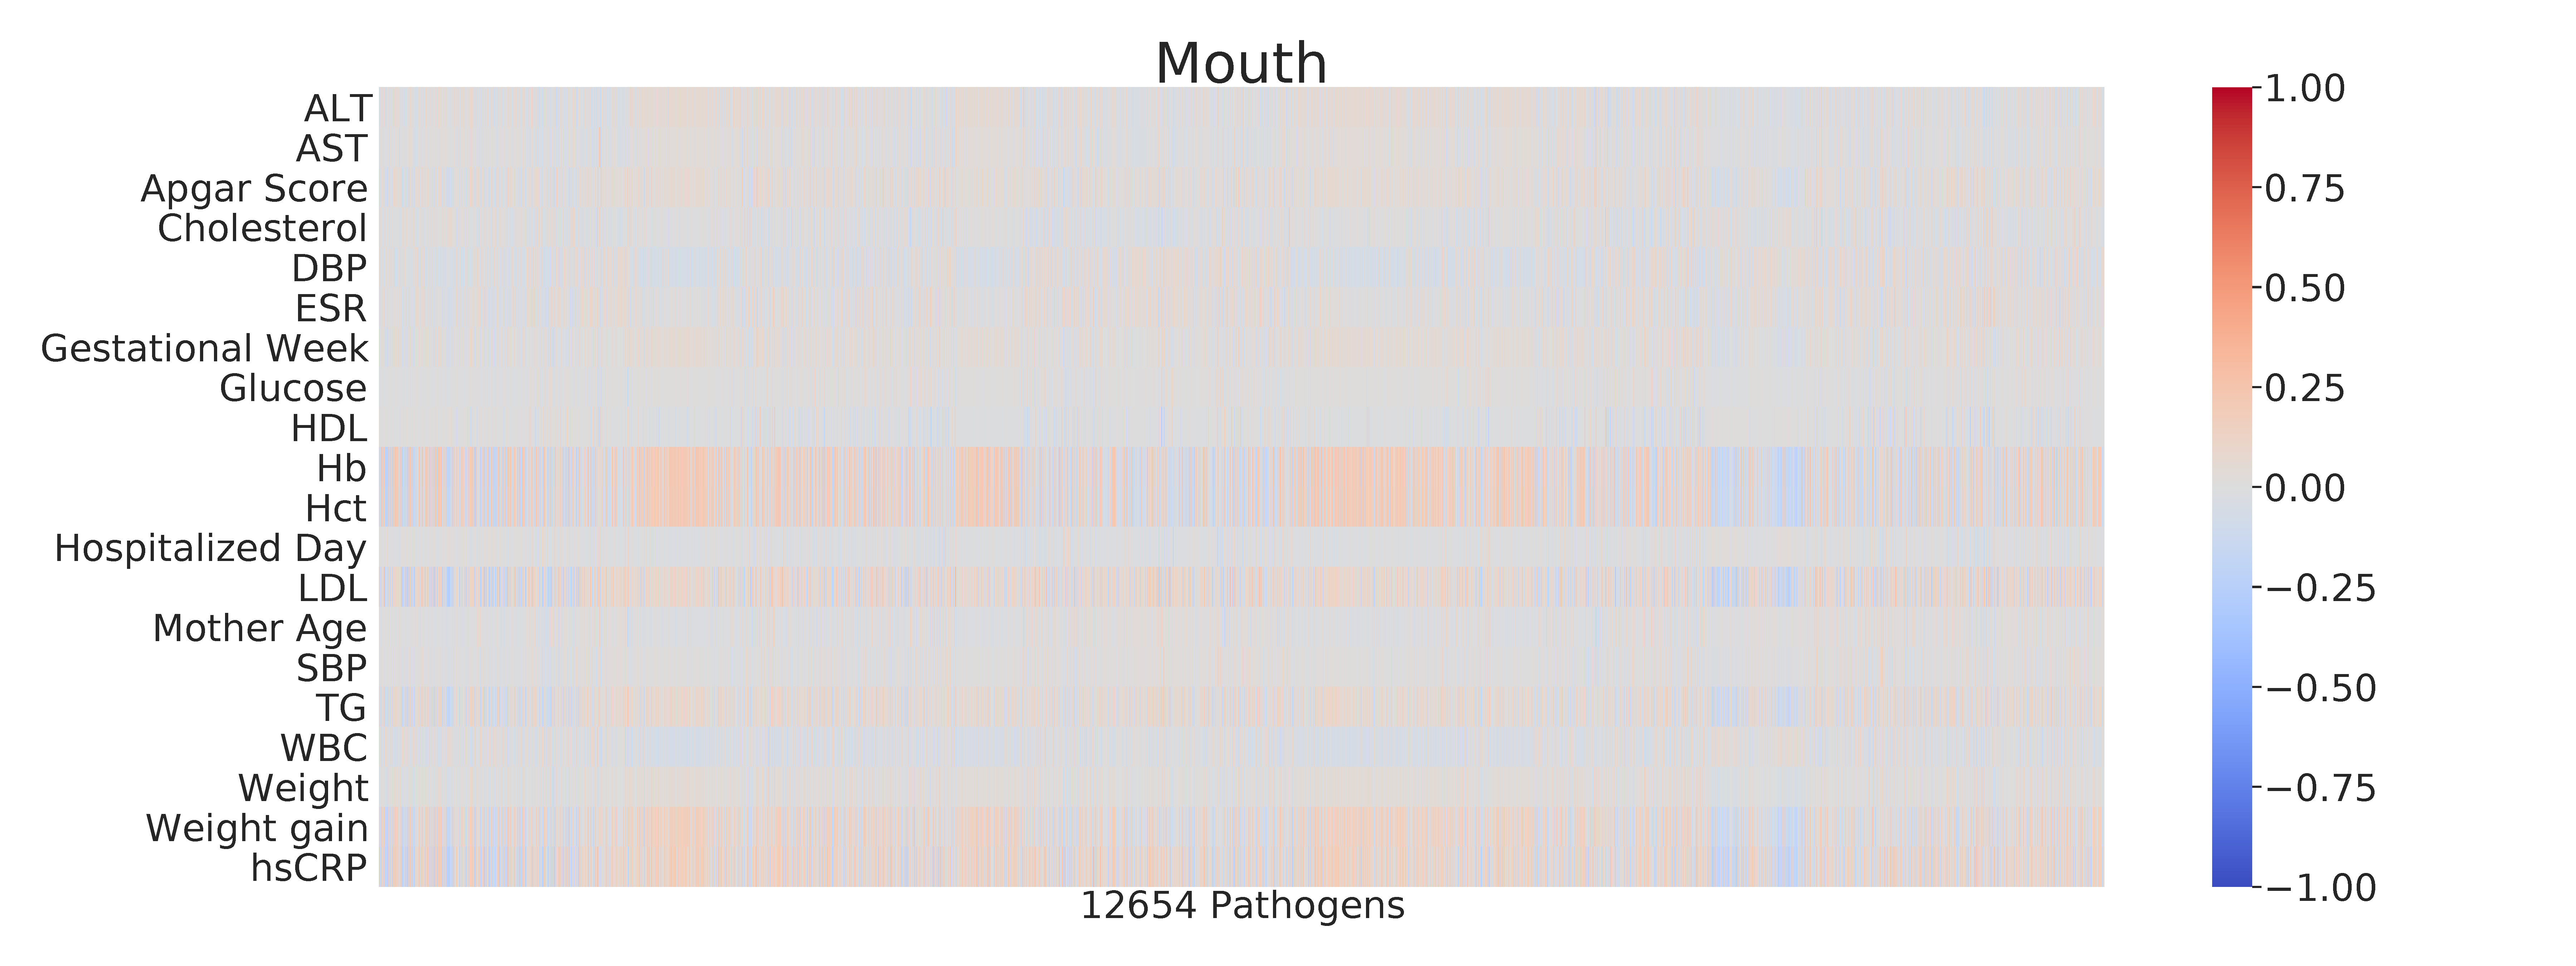
\includegraphics[width=0.7 \linewidth]{figures/Step60_Proportion/singleton.DADA2.homd.uncorrected/Mouth.pdf}
            \caption{Microbial community with Proportion}
        \end{figure}
    \end{frame}

    \begin{frame}[allowframebreaks]
        \frametitle{Notable Taxa}

        \begin{block}{\textit{Streptococcus} spp.}
            \begin{itemize}
                \item \textit{S. mutans}: pathogen of dental caries
                \item Membrane vesicles of Group B \textit{Streptococcus} disrupt feto-maternal barrier \cite{streptococcus-1}. \\
                    $\therefore$ Leading to PTB
            \end{itemize}
        \end{block}

        \begin{block}{\textit{Neisseria} spp.}
            \begin{itemize}
                \item \textit{N.} colonize the mucosal surfaces of many animals.
                \item Only two pathogens in 11 known species
                    \begin{itemize}
                        \item \textit{N. meningitidis}: Meningitis \& Sepsis
                        \item \textit{N. gonorrhoeae}: Gonorrhea (sexual transmitted disease)
                    \end{itemize}
                \item \textit{N. gonorrhoeae} results adverse pregnancy outcomes \cite{neisseria-1}.
            \end{itemize}
        \end{block}

        \begin{block}{\textit{Haemophilus} spp.}
            \begin{itemize}
                \item \textit{H.} inhabit the mucous membranes \\
                    of upper respiratory tract, mouth, vagina, \& intestinal tract.
                \item \textit{H. influenzae}: A major cause of systemic infection
                \item PTB caused by \textit{H. influenzae} \cite{haemophilus-1} and \textit{H. parainfluenzae} \cite{haemophilus-2}.
            \end{itemize}
        \end{block}

        \begin{block}{\textit{R. mucilaginosa}}
            \begin{itemize}
                \item \textit{Rhodotorula mucilaginosa}
                \item \textit{R.} is a genus of pigmented yeasts.
                \item Catheter-related bloodstream infection due to \textit{R. mucilaginosa} \cite{rhodotorula-1}.
                \item $\therefore$ \textit{Rhodotorula} bloodstream infections
            \end{itemize}
        \end{block}

        \begin{block}{\textit{Gemella} spp.}
            \begin{itemize}
                \item \textit{G.} bacteria are primarily found in mucous membranes of human \\
                    \textit{e.g.} oral cavity \& upper digestive tract.
                \item \textit{G. haemolysans} causes endocarditis \cite{gemella-2}.
                \item Women who have PTB also have significant lower level of \textit{G.} \cite{gemella-1}.
            \end{itemize}
        \end{block}
    \end{frame}

    \subsection{Diversity Index}
    \begin{frame}
        \frametitle{Diversity Index}

        \begin{figure}
            \includegraphics[width=0.6 \linewidth]{figures/phylogenic.jpg}
            \caption{Three dimensions of phylogenetic information \protect\cite{phylogenetic1}}
        \end{figure}

        \begin{itemize}
            \item A quantitative measure that shows richness, divergence, and regularity \cite{phylogenetic1}
            \item Alpha diversity: the richness of taxa \textbf{at a single community}
            \item Beta diversity: taxonomy differentiation \textbf{between communities}
        \end{itemize}
    \end{frame}

    \subsubsection{Alpha-diversity}
    \begin{frame}
        \frametitle{Violin Plot with Alpha-diversity}

        \begin{figure}
            \includegraphics[width=0.5 \linewidth]{figures/AlphaDiversity/singleton.DADA2/Mouth+Premature+faith_pd.pdf}
            \caption{Premature \& Faith's PD}
        \end{figure}
    \end{frame}

    \subsubsection{Beta-diversity}
    \begin{frame}[allowframebreaks]
        \frametitle{Beta-diversity t-SNE plots}

        \begin{figure}
            \includegraphics[width=0.5 \linewidth]{figures/BetaDiversity/singleton.DADA2.homd.uncorrected/Mouth+Premature+hamming.pdf}
            \caption{Hamming distance index t-SNE plot}
        \end{figure}
    \end{frame}

    \subsection{Taxonomy Analyses}
    \subsubsection{Differentially Abundant Taxa}
    \begin{frame}
        \frametitle{Volcano plots}

        \begin{figure}
            \includegraphics[width=0.5 \linewidth]{figures/Step44/singleton.DADA2.homd.uncorrected.Mouth.pdf}
            \caption{DAT in Mouth}
        \end{figure}
    \end{frame}

    \begin{frame}[allowframebreaks]
        \frametitle{Violin Plots}

        \begin{columns}
            \begin{column}{0.4 \linewidth}
                \begin{figure}
                    \includegraphics[width=\linewidth]{figures/Step71_Proportion/everything.DADA2.homd.Mouth/C. durum.pdf}
                    \caption{\textit{C. durum}}
                \end{figure}
            \end{column}
            \begin{column}{0.6 \linewidth}
                \begin{block}{\textit{C. durum}}
                    \begin{itemize}
                        \item \textit{Corynebacterium durum}
                        \item Poly-microbial interactions \\
                            $\Rightarrow$ Oral mucosal \& Gingival cells \cite{Corynebacterium-1}.
                        \item Synergism between \textit{C.} \& \textit{Streptococcus} in oral commensals \cite{Corynebacterium-2}.
                    \end{itemize}
                \end{block}
            \end{column}
        \end{columns}

        \begin{columns}
            \begin{column}{0.4 \linewidth}
                \begin{figure}
                    \includegraphics[width=\linewidth]{figures/Step71_Proportion/everything.DADA2.homd.Mouth/P. gingivalis.pdf}
                    \caption{\textit{P. gingivalis}}
                \end{figure}
            \end{column}
            \begin{column}{0.6 \linewidth}
                \begin{block}{\textit{P. gingivalis}}
                    \begin{itemize}
                        \item \textit{Porphyromonas gingivalis}
                        \item \textit{P. gingivalis} is well-known periodontitis pathogen.
                        \item \textit{P. gingivalis} is associated with bacterial vaginosis \cite{Porphyromonas-1}.
                        \item \textit{P. gingivalis} $\Rightarrow$ Adverse prenancy outcomes \cite{Porphyromonas-2}.
                    \end{itemize}
                \end{block}
            \end{column}
        \end{columns}

        \begin{block}{\textit{Prevotella} spp.}
            \begin{itemize}
                \item \textit{P.} spp. interact with human health \cite{Prevotella-1}.
                \item \textit{P.} spp. might have different role in PTB \cite{Prevotella-2}.
                \item \textit{P.} spp. are associated with human infections \cite{Prevotella-4}.
            \end{itemize}
        \end{block}
        \pagebreak

        \begin{columns}
            \begin{column}{0.4 \linewidth}
                \begin{figure}
                    \includegraphics[width=\linewidth]{figures/Step71_Proportion/everything.DADA2.homd.Mouth/P. dentalis.pdf}
                    \caption{\textit{P. dentalis}}
                \end{figure}
            \end{column}
            \begin{column}{0.6 \linewidth}
                \begin{block}{\textit{P. dentalis}}
                    \begin{itemize}
                        \item \textit{Prevotella dentalis}
                        \item \textit{P. dentalis} is observed as colorectal cancer-promoting bacterium \cite{Prevotella-3}.
                    \end{itemize}
                \end{block}
            \end{column}
        \end{columns}

        \begin{columns}
            \begin{column}{0.4 \linewidth}
                \begin{figure}
                    \includegraphics[width=\linewidth]{figures/Step71_Proportion/everything.DADA2.homd.Mouth/P. pleuritidis.pdf}
                    \caption{\textit{P. pleuritidis}}
                \end{figure}
            \end{column}
            \begin{column}{0.6 \linewidth}
                \begin{block}{\textit{P. pleuritidis}}
                    \begin{itemize}
                        \item \textit{Prevotella pleuritidis}
                        \item \textit{P. pleuritidis} causes lung abscess \cite{Prevotella-5}.
                        \item \textit{P. pleuritidis} is abundant in oral microbiome of smokers \cite{Prevotella-6}.
                        \item \textit{P. pleuritidis} associated with gastric cancer \cite{Prevotella-7}.
                    \end{itemize}
                \end{block}
            \end{column}
        \end{columns}
    \end{frame}

    \subsection{Machine Learning}
    \begin{frame}
        \frametitle{ML algorithm comparison}

        \begin{figure}
            \includegraphics[width=\linewidth]{figures/ML.png}
            \caption{Classification Comparison \protect\cite{sklearn1}}
        \end{figure}
    \end{frame}

    \subsubsection{Random Forest Classifier on Proportion}
    \begin{frame}[allowframebreaks]
        \frametitle{Random Forest with (PTB vs. Normal)}

        \begin{figure}
            \includegraphics[width=0.8 \linewidth]{figures/RandomForest_Proportion/singleton-RF.DADA2.homd.Mouth/metrics.pdf}
            \caption{RF evaluations with feature counts}
        \end{figure}

        \begin{figure}
            \includegraphics[width=0.5 \linewidth]{figures/RandomForest_Proportion/singleton-RF.DADA2.homd.Mouth/heatmap.pdf}
            \caption{RF confusion matrix}
        \end{figure}

        \begin{figure}
            \includegraphics[width=0.8 \linewidth]{figures/RandomForest_Proportion/singleton-RF.DADA2.homd.Mouth/importances.pdf}
            \caption{RF importances}
        \end{figure}

        \begin{block}{Highest Importances}
            \begin{enumerate}
                \item \textit{L. umeaense}
                \item \textit{P. gingivalis}
                \item \textit{B.} sp. \textit{HMT 931}
            \end{enumerate}
        \end{block}
    \end{frame}

    \section{Discussion}

    \section{References}
   	\begin{frame}[allowframebreaks]
        \frametitle{References}
        \bibliographystyle{apacite}
        \bibliography{reference}
    \end{frame}
\end{document}